\documentclass{article}

\usepackage[margin=1.6cm]{geometry}
\usepackage{amsmath,amssymb}
\usepackage{float}
\usepackage{graphicx}
\usepackage{fancyhdr}
\pagestyle{fancy}
\usepackage{tcolorbox,listings}
\usepackage{color}
\usepackage{hyperref}
\renewcommand\headrulewidth{1pt}
\usepackage{marvosym}
\usepackage{xcolor}
\usepackage{tikz}
%\usepackage{babel}
\usepackage[french]{babel}
\usepackage[babel=true,kerning=true]{microtype}
\usepackage{afterpage}

\newcommand\myemptypage{
    \null
    \thispagestyle{empty}
    \addtocounter{page}{-1}
    \newpage
    }

\usetikzlibrary{
  arrows,
  calc,
  shapes.geometric,
  shapes.misc,
  shapes.symbols,
  shapes.arrows,
  automata,
  through,
  positioning,
  scopes,
  decorations.shapes,
  decorations.text,
  decorations.pathmorphing,
  shadows}

\definecolor{darkWhite}{rgb}{0.94,0.94,0.94}
 
\lstset{
    backgroundcolor=\color{darkWhite},
    breakatwhitespace=false,
    breaklines=true,
    captionpos=b,
    commentstyle=\color{green},
    deletekeywords={...},
    escapeinside={\%*}{*)},
    extendedchars=true,
    keepspaces=true,
    keywordstyle=\color{blue},
    %language=Python,
    morekeywords={*,...},
    showspaces=false,
    showstringspaces=false,
    showtabs=false,
    stepnumber=1,
    stringstyle=\color{gray},
    tabsize=4,
}
 
\lstdefinestyle{frameStyle}{
    basicstyle=\sffamily,
    numbers=left,
    numbersep=20pt,
    numberstyle=\tiny\color{black}
}
 
\tcbuselibrary{listings,skins,breakable}
 
\newtcblisting{customFrame}{
    arc=0mm,
    top=0mm,
    bottom=0mm,
    left=3mm,
    right=0mm,
    width=\textwidth,
    listing only,
    listing options={style=frameStyle},
    breakable
}

\fancyhead[L]{ALLEMAND Fabien\\COUTURE Louise}
\fancyhead[C]{Modèle de Connaissances\\et Web Sémantique}
\fancyhead[R]{
\includegraphics[scale=0.4]{img/logo_TPS_1.png}}
\fancyfoot[L]{Rapport de Projet}
\fancyfoot[R]{\today}

\begin{document}

\thispagestyle{empty}
\addtocounter{page}{-1}
\begin{center}
	\baselineskip=50pt
	\vspace*{1cm}
	\textbf{{\Huge Modèle de Connaissances\\et Web Sémantique}}\\
	\vspace*{0.25cm}
	\textsf{{\Huge Rapport de Projet}}\\
	\vspace*{0.25cm}
	\begin{minipage}[c]{.46\linewidth}
        \centering
        \textbf{Groupe:}\\
		ALLEMAND Fabien\\
        COUTURE Louise
    \end{minipage}
\end{center}
\vspace{0.1cm}

\begin{figure}[H]
\centering
\centerline{
\includegraphics[scale=2]{img/logo_TPS_2.png}}
\end{figure}

\newpage

\section{Construction de l'Ontologie}

L'objectif de ce projet est de créer une ontologie OWL permettant de représenter le plus précisément possible les informations sur des chansons. Pour cela, nous utilisons le logiciel Protégé développé par l'Université de Stanford ainsi que l'ontologie FOAF (Friend Of A Friend) comme base de notre ontologie.\\
Nous avons tout d'abord créé des classes primitives correspondant aux chansons, aux groupes, aux musiciens (et leurs spécialités) et aux récompenses. 

\begin{figure}[H]
    \center
    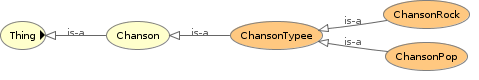
\includegraphics[scale=.5]{img/chanson.png}
    \caption{Hiérarchie des chansons}
\end{figure}

\begin{figure}[H]
    \center
    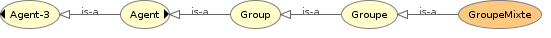
\includegraphics[scale=.5]{img/groupe.png}
    \caption{Hiérarchie des groupes}
\end{figure}

\begin{figure}[H]
    \center
    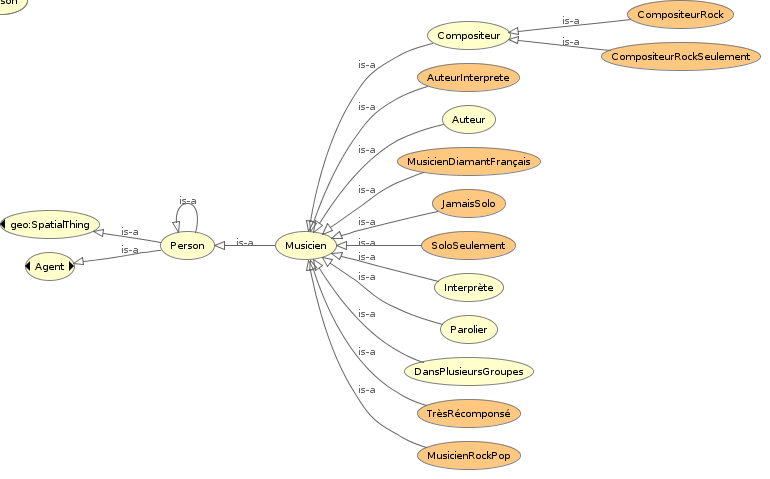
\includegraphics[scale=.5]{img/musicien.png}
    \caption{Hiérarchie des musiciens}
\end{figure}

\begin{figure}[H]
    \center
    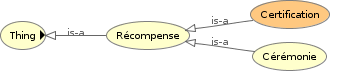
\includegraphics[scale=.5]{img/recompense.png}
    \caption{Hiérarchie des récompenses}
\end{figure}

Il est important de préciser que la plupart des liens sont simples. Par exemple: \textsf{aNationalité} permet d'associer un élément de type \textsf{Person} à une \textsf{Nationalité}. Cependant, afin de traduire l'appartenance d'un artiste à plusieurs groupes, avec des rôles et des périodes données, nous avons du introduire une classe intermédiaire nommée \textsf{ParticipationDansGroupe}. Cette classe peut contenir des assertions qui définissent les dates d'entrée et de sortie du groupe ainsi que le rôle d'un artiste dans ce groupe. Le lien avec le groupe en lui même n'est fait qu'au travers du lien \textsf{aGroupe} qui relie une \textsf{ParticipationDansGroupe} à un \textsf{Groupe}.\\

\begin{figure}[H]
    \centering
    \begin{tikzpicture}[>=stealth,yscale=2,xscale=1.4]
        % Nodes
        \node(musicien) at (0,2)[rectangle,draw,text centered,align=center] {Musicien\\(aNom, aRole)};
        \node(participation) at (0,1)[rectangle,draw,text centered,align=center] {ParticipationDansGroupe\\(aDateDébut, aDateFin, aRoleDansGroupe)};
        \node(groupe) at (0,0)[rectangle,draw,text centered,align=center] {Groupe\\(aNomDeGroupe)};
        % Links
        \draw[->] (musicien) -- (participation) node[midway,right]{participeDansGroupe};
        \draw[->] (participation) -- (groupe) node[midway,right]{aGroupe};
    \end{tikzpicture}
    \caption{Description du lien entre un \textsf{Musicien} et un \textsf{Groupe}} 
\end{figure}

Nous avons aussi ajouté diverses classes définies pour répondre à nos besoins.

\section{Interrogation de l'Ontologie}
Nous avons par la suite pu interroger l'ontologie à l'aide de requêtes SPARQL et SQWRL. Par commodité, les requêtes demandées sont écrites dans le fichier \path{AllemandCouture_Requetes.md}. Voici deux exemples de requêtes qui étaient demandées.\\

La première est une requête SPARQL qui retrouve les groupes ayant prublié moins de 4 albums et affiche le groupe ainsi que le nombre d'albums publiés. On remarque l'utilisation d'une instruction \textsf{GROUP BY} pour que la fonction \textsf{count} regroupe le calcul par groupe. L'instruction \textsf{HAVING} agit comme un filtre, ici, élimine les groupes ayant publié au moins 4 albums.

\begin{lstlisting}[H]
    SELECT ?g (count(distinct ?a) as ?count)
    WHERE {?a rdf:type ch:Album .
           ?g ch:aPublié ?a }
    GROUP BY (?g)       # Regrouper le résultat par groupe
    HAVING (?count < 4) # Conserver les groupes dont le résultat est inférieur à 4 
    \end{lstlisting}

La deuxième requête permet de lister chaque participation d'un artiste dans un groupe. On observe en sortie le nom de l'artiste et le groupe. Les trois premières instructions permettent de lier chaque artiste à un groupe et les deux dernières récupèrent le nom de l'artiste et du groupe.

\begin{lstlisting}[H]
Musicien(?m) ^ participeDansGroupe(?m, ?p) ^ aGroupe(?p, ?g) ^ aNom(?m, ?n) ^ aNomDeGroupe(?g, ?ng) -> sqwrl:select(?n, ?ng)
\end{lstlisting}

\end{document}